\documentclass[english,brazil,notheorems]{beamer}
\usepackage[utf8]{inputenc}
\usepackage{babel}
\usepackage{latexsym}
\usepackage{amsmath}
\usepackage{amssymb}
\usepackage{graphicx}
\usepackage{amsfonts,amscd,bezier,amssymb} %Pacotes matemáticos
\usepackage{amsmath, amsthm} %Outros pacotes matemáticos
\usepackage[mathscr]{eucal} %Outros pacotes matemáticos
\usepackage{algpseudocode} %Pacote de algoritmos
\usepackage[ruled]{algorithm} %Pacote de algoritmos
%\usepackage{algorithmicx} %Pacote de algoritmo
\usepackage{pgfpages}
\usepackage{subfig}
\usepackage{wasysym}
\usepackage{multicol}
\usepackage{listingsutf8}

\newcommand\ASTART[1][]{\bigskip\noindent\begin{minipage}[c]{0.5\linewidth}}
\newcommand\ACONTINUE[1][]{\end{minipage}\begin{minipage}[c]{0.5\linewidth}}
\newcommand\AENDSKIP{\end{minipage}\bigskip}
\newcommand\AEND{\end{minipage}}

\usepackage[justification=centering]{caption}
\ifx\hypersetup\undefined
  \AtBeginDocument{%
    \hypersetup{unicode=true}
  }
\else
  \hypersetup{unicode=true}
\fi
\let\Tiny=\tiny


\usetheme{boxes}
\usecolortheme{orchid}
\usefonttheme{professionalfonts}

\setbeamercovered{transparent}
% or whatever (possibly just delete it)

\newtheorem{theorem}{Teorema}
\newtheorem{lemma}[theorem]{Lema}
\newtheorem{corollary}[theorem]{Corolário}
\newtheorem{proposition}[theorem]{Proposição}
\newtheorem{example}[theorem]{Exemplo}
\theoremstyle{definition}
\newtheorem{deffinition}[theorem]{Definição}
\newtheorem{obs}[theorem]{Observação}

% \floatname{algorithm}{Algoritmo}
% \algrenewcommand\algorithmicrequire{\textbf{Entrada:}}
% \algrenewcommand\algorithmicensure{\textbf{Saída:}}
% \algrenewcommand\algorithmicprocedure{\textbf{procedimento}}
% \algrenewcommand\algorithmicfunction{\textbf{função}}
% \algrenewcommand\algorithmicif{\textbf{se}}
% \algrenewcommand\algorithmicthen{\textbf{então}}
% \algrenewcommand\algorithmicelse{\textbf{senão}}
% \algrenewcommand\algorithmicwhile{\textbf{enquanto}}
% \algrenewcommand\algorithmicdo{\textbf{faça}}
% \algrenewcommand\algorithmicend{\textbf{fim}}
% \algrenewcommand\algorithmicreturn{\textbf{retorne}}

\definecolor{dkgreen}{rgb}{0,0.6,0}
\definecolor{blue}{rgb}{0.5,0.5,0.5}
\definecolor{mauve}{rgb}{0.58,0,0.82}

\lstdefinestyle{codeC}{
 inputencoding = utf8x,
 language=C,
 basicstyle=\scriptsize,
 %frame=tb,
 numbers=left,
 numberstyle=\tiny,
 columns=fullflexible,
 extendedchars=true,
 morekeywords={\%* },
 showstringspaces=false
 keywordstyle=\color{blue},
 commentstyle=\color{dkgreen},
 stringstyle=\color{mauve},
 escapeinside={\%*}{*)},
 breaklines = true, % Configura quebra de linha automática
}

\newcommand{\R}{\mathbb{R}}
\newcommand{\Z}{\mathbb{Z}}
\newcommand{\N}{\mathbb{N}}
\newcommand{\cor}{\operatorname{cor}}


%
\mode<presentation>
{
  \usetheme{default}      % or try Darmstadt, Madrid, Warsaw, ...
  \usecolortheme{default} % or try albatross, beaver, crane, ...
  \usefonttheme{default}  % or try serif, structurebold, ...
  \setbeamertemplate{navigation symbols}{}
  \setbeamertemplate{caption}[numbered]
} 

% \AtBeginSection[]{
%    \frame<beamer>{ 
%    \frametitle{Sumário}   
%    \tableofcontents[currentsection,currentsubsection] 
%   }
% }


%\pgfpagesuselayout{resize to}[physical paper width=8in, physical paper height=6in]

\title[Introdução ao \LaTeX]{Introdução ao sistema de tipografia \LaTeX}
%\subtitle{}
\author[Alexsander Melo \and Ygor Canalli]{Alexsander~Melo\and Ygor~Canalli}
\institute[UFRRJ]{Departamento de Ciência da Computação\\Universidade Federal Rural do Rio de Janeiro}
\date[UFRRJ 2014]{UFRRJ, Outubro de 2014}


\begin{document}

\begin{frame}
  \titlepage
\end{frame}

\begin{frame}{Sumário}
  \tableofcontents{}
\end{frame}

\section{O que é o \LaTeX}
%\subsection{\TeX}

\begin{frame}{O que é o \TeX}
\visible<2->{
\begin{figure}
  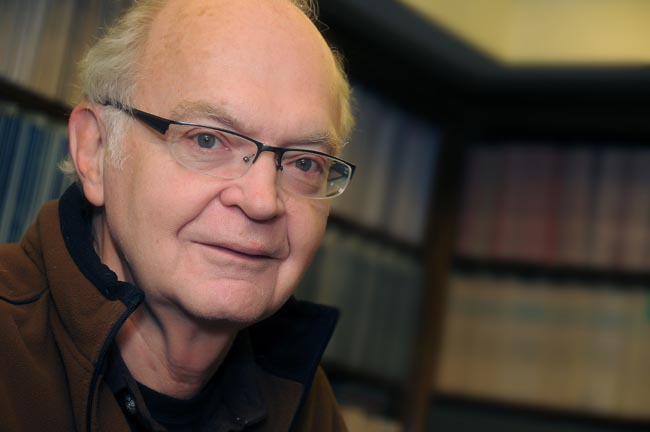
\includegraphics[scale=0.35]{Imagens/knuth.jpg}
  \caption{Donald Knuth}
 \end{figure}
}
\end{frame}

\begin{frame}{O que é o \TeX}
 \begin{itemize}
 \item<1->{O \TeX~(lê-se téc) é um programa de computador para processamento de texto e formulas matemáticas.}
 
 \item<2->{Em 1977 o cientista \alert<3->{Donald E. Knuth} impelido por uma insatisfação com a deterioração da qualidade tipográfica de seus próprios livros, diante das primeiras impressoras digitais que surgiam, decidiu escrever um programa capaz de solucionar seus problemas.}
 
 \item<4->{O software teve sua principal versão lançada em 1982, mas só em 1989 passou a dar suporte sólido para caracteres de 8 bits.}
 
 \item<5->{Desde então o \TeX~passou a ser amplamente utilizado, subretudo pela comunidade científica, para tipografia digital de texto e fórmulas matemáticas.}
\end{itemize}
\end{frame}


%\subsection{\LaTeX}
\begin{frame}{O que é o \LaTeX}
\visible<2->{
\begin{figure}
  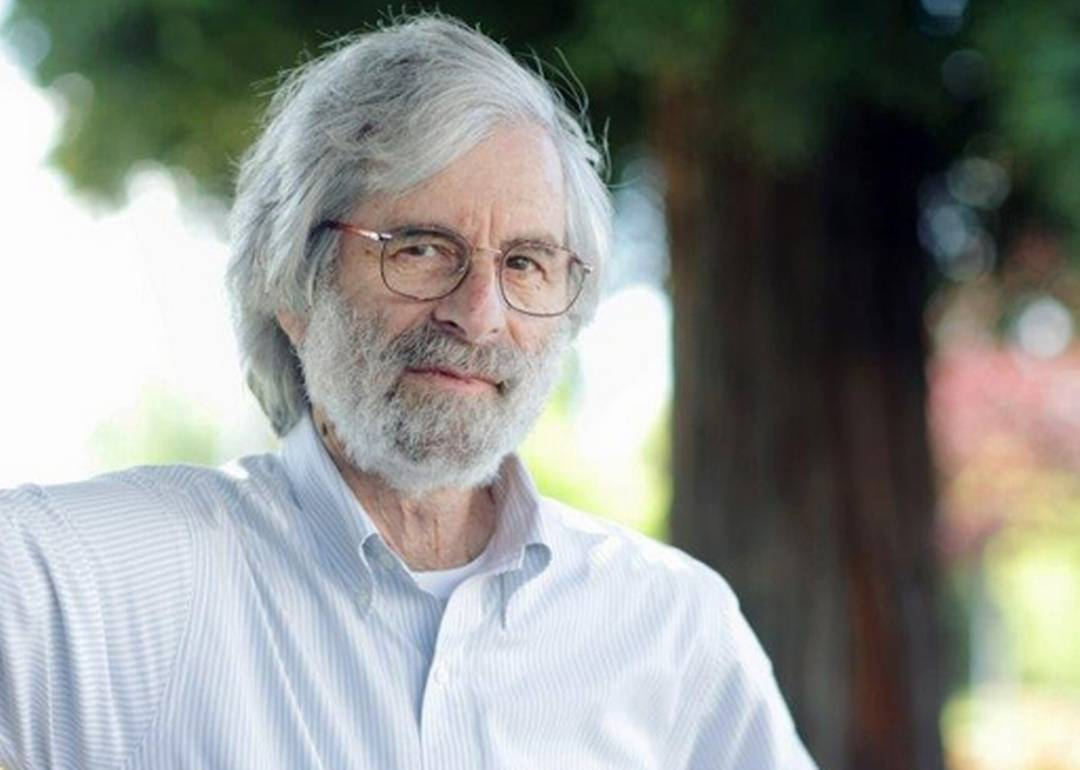
\includegraphics[scale=0.15]{Imagens/lamport.jpg}
  \caption{Leslie Lamport}
 \end{figure}
}
\end{frame}

\begin{frame}{O que é o \LaTeX}
\begin{itemize}
 
 \item O \LaTeX~é um sistema tipográfico de alta qualidade voltado para escrita de documentação técnica e científica que fornece um conjunto de \emph{macros} que possibilita processar e imprimir trabalhos utilizando um \emph{layout} pré-definido.
 
 \item<2->{O \LaTeX~foi originalmente desenvolvido pelo pesquisador \alert<3->{Leslie~Lamport} e se utiliza do \TeX~como mecanismo de processamento. A versão original de Lamport é constantemente aprimorada e corrigida por uma comunidade de voluntários que mantém o software livre.}

\end{itemize}
\end{frame}

%\subsection{Diferença dos programas de processamento de texto}
% \begin{frame}{Diferença dos programas de processamento de texto}
%  
% \end{frame}

%\subsection{Porque usar \LaTeX}
\begin{frame}{Porque usar \LaTeX}

  \begin{itemize}
  \item Facilidade de escrever expressões matemáticas
  \pause
  \item Qualidade do resultado final
  \pause
  \item Possibilidade de incorporar \emph{layouts}
  \pause
  \item Foco na estrutura do texto ao invés da formatação
  \pause
  \item Automatização de numerações e referencias
  \pause
  \item Encoraja a escrita de textos bem estruturados
  \pause
  \item Estabilidade e compatibilidade
  \pause
  \item É divertido! \smiley
  \end{itemize}

\end{frame}

%\subsection{Desvantagens do \LaTeX}
\begin{frame}{Desvantagens do \LaTeX}
  \begin{itemize}
  \item Interface não convencional (“what you see is what you get”, ou simplesmente WYSIWYG)
  \pause
  \item Necessidade de resolver dependência de pacotes
  \pause
  \item O desenvolvimento de um novo \emph{layout} (classe) inteiro é difícil
  \pause
  \item Necessidade eventual de debugar \frownie
  \end{itemize}
\end{frame}

% \section{Noções básicas}
% \begin{frame}{Noções básicas}
% 
% \end{frame}

%\subsection{Estrutura de um arquivo de entrada}
\begin{frame}[fragile]{Estrutura de um arquivo de entrada}
 \begin{verbatim}
\documentclass[a4paper,10pt]{article}
\usepackage[utf8]{inputenc}

%opening
\title{}
\author{}

\begin{document}
\maketitle

\begin{abstract}
\end{abstract}

\section{}
\end{document}
\end{verbatim}
\end{frame}

\begin{frame}[fragile]{O Preâmbulo}
\begin{itemize}
 \item É considerado \alert<1->{preâmbulo} de um arquivo \LaTeX~tudo que estiver contido entre os comandos $\backslash$\verb|documentclass| e \verb|\begin{document}|.
  
 \item<2->{A sintaxe do comando $\backslash$\verb|documentclass| é dada da seguinte forma:}

 \pause
 \begin{center}
    $\backslash$\verb|documentclass[options]{class}|
 \end{center}

 \item<4->{\bf options:}
 \begin{itemize}
  \item tamanho do papel (\texttt{a4paper})
  \item tamanho da fonte
  \item orientação do documento (retrato / paisagem)
 \end{itemize}
 
 \item<5->{\bf class:}
 \begin{multicols}{2}
 \begin{itemize}
  \item article
  \item book
  \item slide
  \item beamer
  \item report
  \item letter
 \end{itemize}
\end{multicols}
\end{itemize}
\end{frame}

\begin{frame}[fragile]{O Prêambulo}
\begin{itemize}
 \item A diretiva $\backslash$\verb|usepackage{name}| permite que pacotes sejam carregados ao documento $\LaTeX$ sendo editado, permitindo então um aumento considerável da capacidade de formatação do $\LaTeX$.
 \item<2->{Um exemplo, ao se carregar o pacote \verb|graphicx|, permite-se que sejam carregas imagens e gráficos no documento sendo editado, isto se dá através do comando: $\backslash$\verb|usepackage{graphicx}|.}
\end{itemize}
\end{frame}

%\subsection{Espaçamento}
% \begin{frame}{Espaçamento}
%   
% \end{frame}
% 
% %\subsection{Comandos}
\begin{frame}{Comandos}
  Os comando do \LaTeX~são \emph{case sensitive}, isto é, diferem caracteres maiúsculos de minúsculos e seguem um dos dois formatos:
  
  \begin{itemize}
   \item Começam com uma contra-barra ($\backslash$) e possuem um nome que consiste apenas em letras. Os comandos são terminados por um espaço, um número ou qualquer outro caractere que não seja letra.
   \item Uma contra-barra e apenas um caracter especial 
  \end{itemize}
\end{frame}


% %\subsection{Caracteres es
% peciais}
 \begin{frame}[fragile]{Caracteres especiais}
 \begin{center}
  \begin{table}
    \begin{tabular}{|c|c|}
     \hline
     Caracter & Comando \\
     \hline
     \# & $\backslash$\# \\
     \$ & $\backslash$\$ \\
     \% & $\backslash$\% \\
     \^{} & $\backslash$\^{} \\
     \& & $\backslash$\& \\
     \_ & $\backslash$\_ \\
     \{ & $\backslash$\{ \\
     \} & $\backslash$\} \\
     \~{} & $\backslash$\~{} \\
     $\backslash$ & \verb:$\backslash$: \\
     \hline
   \end{tabular}
 \end{table}
 \end{center}
\end{frame}
% 
%\subsection{Ambientes}
\begin{frame}[fragile]{Ambientes}

Defini-se ambiente todo comando com a estrutura
 
  \begin{verbatim}
  \begin{ambiente}
  ...
  \end{ambiente}
 \end{verbatim}
 
Ambientes podem ser aninhados, desde que respeitem as respectivas aberturas e fechamentos, como segue:

  \begin{verbatim}
  \begin{ambienteA}
    ...    
    \begin{ambienteB}
      ...
    \end{ambienteB}
    ...
  \end{ambienteA}
 \end{verbatim}

\end{frame}

%\subsection{Comentários}
\begin{frame}[fragile]{Comentários}
 No \LaTeX~os comentários podem ser feitos através do caracter especial \verb:%:, ou através do ambiente \verb:comment: incluído no pacote \emph{verbatim} (\verb:\usepackage{verbatim}:) 
 \begin{verbatim}
  \begin{comment}
    Seu comentário
    de múltiplas linhas
    pode ser feito desta forma!
  \end{comment}
 \end{verbatim}
\end{frame}

\section{Capítulos, Seções e Subseções}

%\subsection{Trabalhando com capítulos, seções, subseções, etc.}
\begin{frame}[fragile]{Trabalhando com capítulos, seções, subseções, etc.}
 \begin{enumerate}
 \item Capítulos são declarados com o comando \verb:\chapter{Nome do capítulo}: (disponível apenas em documentos do tipo \emph{book})
 \pause
 \item Seções são declarados com o comando \verb:\section{Nome da seção}:
 \pause
 \item Subseções são declarados com o comando \verb:\subsection{Nome da subseção}:
 \pause
 \item Subsubseções são declarados com o comando \verb:\subsubsection{Nome da subsubseção}:

 \end{enumerate}

\end{frame}

\section{Formatando texto}

%\subsection{Tipos e tamanhos de letras}
\begin{frame}[fragile]{Tipos e tamanhos de letras}
  \begin{center}
  \begin{table}
    \begin{tabular}{|c|c|}
     \hline
     Comando & Efeito \\
     \hline
     \verb:{\rm Romano}: & {\rm Romano} \\
     \verb:{\bf Negrito}: & {\bf Negrito} \\
     \verb:{\sl Inclinado}: & {\sl Inclinado} \\
     \verb:{\sf Sans Serif}: & {\sf Sans Serif} \\
     \verb:{\it Italico}: & {\it Italico} \\
     \verb:{\sc Caixa Alta}: & {\sc Caixa Alta} \\
     \verb:{\tt Monospace}: & {\tt Monospace}\\
     \hline
   \end{tabular}
 \end{table}
 \end{center}
\end{frame}

\begin{frame}[fragile]{Tipos e tamanhos de letras}
  \begin{center}
  \begin{table}
    \begin{tabular}{|c|c|}
     \hline
     Comando & Efeito \\
     \hline
     \verb:{\tiny Tamanho}: & {\tiny Tamanho} \\
     \verb:{\scriptsize Tamanho}: & {\scriptsize Tamanho} \\
     \verb:{\footnotesize Tamanho}: & {\footnotesize Tamanho} \\
     \verb:{\small Tamanho}: & {\small Tamanho} \\
     \verb:{\normalsize Tamanho}: & {\normalsize Tamanho} \\
     \verb:{\large Tamanho}: & {\large Tamanho} \\
     \verb:{\Large Tamanho}: & {\Large Tamanho}\\
     \verb:{\LARGE Tamanho}: & {\LARGE Tamanho}\\
     \verb:{\huge Tamanho}: & {\huge Tamanho}\\
     \verb:{\Huge Tamanho}: & {\Huge Tamanho}\\
     \hline
   \end{tabular}
 \end{table}
 \end{center}
\end{frame}

%\subsection{Acentuação}
\begin{frame}[fragile]{Acentuação}
\begin{itemize}
 \item Originalmente, a acentuação em \LaTeX~é feita através de uma contra-barra seguida do acento e da letra (por exemplo $\backslash$\verb|'{a}| refere-se ao \'{a}), exceto o cedilha, que é construído com um \c seguido de um outro c, isto é, $\backslash$\verb|c{c}|.
 
 \item<2->{Como a língua portuguesa possui muita acentuação, este processo todo se torna considerável custoso... \frownie} 
 
 \vspace{2ex}
 
 \item<3->{\verb|\usepackage[utf8]{inputenc}| \smiley.}
 
 \item<4->{Além do inputec, existe também o pacote \verb|babel| que facilita trabalhar em \LaTeX~com múltiplas linguagens, por exemplo, ao hifenizar palavras automaticamente.}
 
 \item<5->{\verb|\usepackage[brazil]{babel}|.}
\end{itemize}
\end{frame}

%\subsection{Alinhamento de texto}
\begin{frame}[fragile]{Alinhamento de texto}
 \begin{itemize}
  \item
  \ASTART
    Alinhamento centralizado
  \ACONTINUE
    \begin{verbatim}
     \begin{center}
      ...
     \end{center}
    \end{verbatim}
  \AEND

  \item
  \ASTART
    Alinhamento à esquerda
  \ACONTINUE
    \begin{verbatim}
     \begin{flushleft}
      ...
     \end{flushleft}
    \end{verbatim}
  \AEND
 
 \item
  \ASTART
    Alinhamento à direita
  \ACONTINUE
    \begin{verbatim}
     \begin{flushright}
      ...
     \end{flushright}
    \end{verbatim}
  \AEND
 \end{itemize}
\end{frame}

%\subsection{Ambiente tabular}
\begin{frame}[fragile]{Ambiente tabular}
 \begin{center}
  \ASTART
 \begin{tabular}{cc}
      a & b \\
      c & d
 \end{tabular}
\ACONTINUE
 \begin{verbatim}
  \begin{tabular}{cc}
      a & b \\
      c & d
 \end{tabular}
 \end{verbatim}
\AEND

\ASTART
 \begin{tabular}{|c|c|}
      \hline 
      a & b \\ \hline
      c & d \\ \hline
 \end{tabular}
\ACONTINUE
 \begin{verbatim}
 \begin{tabular}{|c|c|}
      \hline \\
      a & b 
      \hline \\
      c & d
      \hline
 \end{tabular}
 \end{verbatim}
\AEND
 \end{center}
\end{frame}


\begin{frame}[fragile]{Ambiente tabular}
 \begin{center}\footnotesize
 \begin{tabular}{r|cl}
      Algoritmo		& Desempenho	& Comentário \\
      \hline
      Bubble-sort	& Péssimo	& Algoritmo com complexidade mais alta \\
      Insertion-sort	& Regular	& Ótimo desempenho para inserções constantes \\
      Merge-sort	& Ótimo		& Alto consumo de memória \\
      Quick-sort	& Ótimo		& Quase sempre a melhor escolha
 \end{tabular} 

 \vspace{2ex}
 \scriptsize
 \begin{verbatim}
 \begin{tabular}{r|cl}
      Algoritmo		& Desempenho	& Comentário \\
      \hline
      Bubble-sort	& Péssimo	& Algoritmo com complexidade mais alta \\
      Insertion-sort	& Regular	& Ótimo desempenho para inserções constantes \\
      Merge-sort	& Ótimo		& Alto consumo de memória \\
      Quick-sort	& Ótimo		& Quase sempre a melhor escolha
 \end{tabular} 
 \end{verbatim}
 \end{center}
\end{frame}

\section{Listas, Enumerações e descrições}
\begin{frame}[fragile]{Listas, Enumerações e descrições}
 \begin{center}
\ASTART
 \begin{itemize}
      \item Este é um item
      \item Outro item
      \item Mais um item
 \end{itemize} 
\ACONTINUE
 \begin{verbatim}
 \begin{itemize}
      \item Este é um item
      \item Outro item
      \item Mais um item
 \end{itemize} 
 \end{verbatim}
\AEND

\ASTART

 \begin{itemize}
    \item Este é um item
    \begin{itemize}
	\item Subitem
	\item Outro subitem
    \end{itemize}
    \item Mais um item
 \end{itemize}
\ACONTINUE
 \begin{verbatim}
 \begin{itemize}
    \item Este é um item
    \begin{itemize}
      \item Subitem
      \item Outro subitem
    \end{itemize}
    \item Mais um item
 \end{itemize}
 \end{verbatim}
\AEND
\end{center}
\end{frame}

\begin{frame}[fragile]{Listas, Enumerações e descrições}
 \begin{center}
\ASTART
 \begin{enumerate}
      \item Este é um item
      \item Outro item
      \item Mais um item
 \end{enumerate} 
\ACONTINUE
 \begin{verbatim}
 \begin{enumerate}
      \item Este é um item
      \item Outro item
      \item Mais um item
 \end{enumerate} 
 \end{verbatim}
\AEND

\ASTART
 \begin{enumerate}
    \item Este é um item
    \begin{enumerate}
	\item Subitem
	\item Outro subitem
    \end{enumerate}
    \item Mais um item
 \end{enumerate}
\ACONTINUE
 \begin{verbatim}
 \begin{enumerate}
    \item Este é um item
    \begin{enumerate}
      \item Subitem
      \item Outro subitem
    \end{enumerate}
    \item Mais um item
 \end{enumerate}
 \end{verbatim}
\AEND
\end{center}
\end{frame}

\begin{frame}[fragile]{Listas, Enumerações e descrições}
 \begin{center}
 \ASTART\scriptsize
 \begin{description}
    \item [Teste a:] resultado x
    \item [Teste b:] resultado y
 \end{description}
\ACONTINUE\scriptsize
 \begin{verbatim}
 \begin{description}
    \item [Teste a:] resultado x
    \item [Teste b:] resultado y
 \end{description}
 \end{verbatim}
\AEND
\end{center}
\end{frame}


\section{Textos matemáticos}

\begin{frame}[fragile]{Textos matemáticos}
 Todo conteúdo entre dois caracteres \$ será reconhecido como uma expressão matemática em linha.
\scriptsize
\ASTART
$y = ax + b$
\ACONTINUE
\verb:$y = ax + b$:
\AEND

\ASTART
$a^2 = b^2 + c^2$
\ACONTINUE
\verb:$a^2 = b^2 + c^2$:
\AEND

\ASTART
$a^{2i} * b_j / c_{j-1}$
\ACONTINUE
\verb:$a^{2i} * b_j / c_{j-1}$:
\AEND

\ASTART
$\frac{1}{x} \cdot ( \frac{2k}{\omega} - \delta )$
\ACONTINUE
\begin{verbatim}
 $\frac{1}{x} \cdot
 ( \frac{2k}{\omega} - \delta )$
\end{verbatim}

\AEND

\ASTART
$\sum\limits_{i=1}^{n} C_i d_i$
\ACONTINUE
\verb:$\sum\limits_{i=1}^{n} C_i d_i$:
\AEND

\ASTART
$\int\limits_{-\infty}^{\infty} \varepsilon dx$
\ACONTINUE
\begin{verbatim}
$\int\limits_{-\infty}^{\infty}
 \varepsilon dx$
\end{verbatim}
\AEND
\end{frame}

\begin{frame}[fragile]{Textos matemáticos}
 Também é possível expandir expressões como $\frac{1}{x} \cdot \frac{2k}{\omega} - \delta $ para uma linha própria da seguinte forma \[\frac{1}{x} \cdot \frac{2k}{\omega} - \delta\] substituindo os delimitadores \$ \, \$ por \verb:\[  \]:
\end{frame}

\begin{frame}[fragile]{Textos matemáticos}
 
Certas vezes parenteses, colchetes e chaves não se ajustam bem a uma expressão:
\[x = [\frac{1}{x} \cdot (\frac{2k}{\omega} - \delta)]. \]

{\scriptsize \verb:\[x = [\frac{1}{x} \cdot (\frac{2k}{\omega} - \delta)] \]:}

\vspace{1ex}
Nesses casos eles podem ser ajustados ao tamanho de uma expressão para uma melhor visualização:

\[x = \left[ \frac{1}{x} \cdot \left( \frac{2k}{\omega} - \delta \right) \right] \]

\scriptsize
\begin{verbatim} 
 \[x = \left[ \frac{1}{x} \cdot 
 \left( \frac{2k}{\omega} - \delta \right) \right] \]
\end{verbatim}

\end{frame}

\begin{frame}[fragile]{Textos matemáticos}

Podemos criar equações referenciáveis através do ambiente \verb:equation: combinado com o comando \verb:label:, como a que segue
\begin{equation} \label{minha_equacao}
\lim_{x \to \infty} \frac{1}{x}.
\end{equation}

A equação~\eqref{minha_equacao} foi criada através do código 

\begin{center}
\scriptsize
 \begin{verbatim}
\begin{equation} \label{minha_equacao}
  \lim_{x \to \infty} \frac{1}{x}
\end{equation}
\end{verbatim}
\end{center}

e foi referenciada através do comando \emph{eqref} da seguinte forma:~\verb:\eqref{minha_equacao}:.

\end{frame}

%\subsection{Matrizes e sistemas}
\begin{frame}[fragile]{Matrizes e sistemas}
\ASTART
 \begin{displaymath}
 A = \left[
  \begin{array}{ccc}
   1 & 0 & 4 \\
   9 & 2 & 7 \\
   0 & 0 & 3
  \end{array}
  \right]
 \end{displaymath}
\ACONTINUE
 \begin{displaymath}
  \left\{
  \begin{array}{rclcl}
   x & = & 2 & + & y \\
   y & = & z & + & x \\
   7z & = &2\omega & + & \pi
  \end{array}
  \right.
 \end{displaymath}
\AEND

\vspace{1ex}

\scriptsize
\ASTART
\begin{verbatim}
 \begin{displaymath}
 A = \left[
  \begin{array}{ccc}
   1 & 0 & 4 \\
   9 & 2 & 7 \\
   0 & 0 & 3
  \end{array}
  \right]
 \end{displaymath}
\end{verbatim}
\ACONTINUE
\begin{verbatim}
 \begin{displaymath}
  \left\{
  \begin{array}{rclcl}
   x & = & 2 & + & y \\
   y & = & z & + & x \\
   7z & = &2\omega & + & \pi
  \end{array}
  \right.
 \end{displaymath}
\end{verbatim}
\AEND

\end{frame}


\section{Algoritmos e Códigos}
\begin{frame}{Algoritmos}
  \begin{algorithm}[H]
  \caption{Algoritmo de Euclides}
  \begin{algorithmic}[1]
   \Require $a, b \in \N$
   \Ensure $\gcd(a, b)$
   \Function{Euclides}{$a, b$}
     \If {$(b == 0)$}
      \State \Return $a$
     \Else \State \Return {\sc Euclides}$(b$, $a \bmod b)$
     \EndIf
   \EndFunction
  \end{algorithmic}
 \end{algorithm}
\end{frame}

\begin{frame}[fragile]{Algoritmos}
\scriptsize
\begin{verbatim}
\usepackage{algpseudocode}
\usepackage[ruled]{algorithm}

\begin{algorithm}[H]
  \caption{Algoritmo de Euclides}
  \begin{algorithmic}[1]
   \Require $a, b \in \N$
   \Ensure $\gcd(a, b)$
   \Function{Euclides}{$a, b$}
     \If {$(b == 0)$}
      \State \Return $a$
     \Else \State \Return {\sc Euclides}$(b$, $a \bmod b)$
     \EndIf
   \EndFunction
  \end{algorithmic}
 \end{algorithm}
\end{verbatim}
\end{frame}

\begin{frame}{Algoritmos}
  \begin{algorithm}[H]\footnotesize
    \begin{algorithmic}[1]
      \Require Strings: $s$, $t$, Tamanhos: $len_s$, $len_t$, Custos: $ic, rm, sc$.
      \Function{levenshtein}{$s$, $len_s$, $t$, $len_t$}
	\State Incializa $d[0..len_s][0..len_t]$
	\For {$i = 0$ \text{\bf até} $len_s + 1$}
	  \State d[i][0] = i
	\EndFor
	\For {$j = 0$ \text{\bf até} $len_t + 1$}
	  \State d[0][j] = j
	\EndFor
	\For {$i = 1$ \text{\bf até} $len_s + 1$}
	  \For {$j = 1$ \text{\bf até} $len_t + 1$}
	    \If {$s[i-1] == t[j-1]$}
		\State $d[i][j] = min(d[i-1][j] + rc, d[i][j-1] + ic, d[i-1][j-1]$)
		\Else
		  \State $d[i][j] = min(d[i-1][j] + rc, d[i][j-1] + ic, d[i-1][j-1] + sc$)
		\EndIf
	  \EndFor
	\EndFor
	\EndFunction
    \end{algorithmic}
  \end{algorithm}
 \end{frame}

\begin{frame}[fragile]{Algoritmos}
\tiny
\begin{verbatim}
\begin{algorithm}[H]
   \begin{algorithmic}[1]
      \Require Strings: $s$, $t$, Tamanhos: $len_s$, $len_t$, Custos: $ic, rm, sc$.
      \Function{levenshtein}{$s$, $len_s$, $t$, $len_t$}
	\State Incializa $d[0..len_s][0..len_t]$
	\For {$i = 0$ \text{\bf até} $len_s + 1$}
	  \State d[i][0] = i
	\EndFor
	\For {$j = 0$ \text{\bf até} $len_t + 1$}
	  \State d[0][j] = j
	\EndFor
	\For {$i = 1$ \text{\bf até} $len_s + 1$}
	  \For {$j = 1$ \text{\bf até} $len_t + 1$}
	    \If {$s[i-1] == t[j-1]$}
		\State $d[i][j] = min(d[i-1][j] + rc, d[i][j-1] + ic, d[i-1][j-1]$)
		\Else
		  \State $d[i][j] = min(d[i-1][j] + rc, d[i][j-1] + ic, d[i-1][j-1] + sc$)
		\EndIf
	  \EndFor
	\EndFor
	\EndFunction
    \end{algorithmic}
  \end{algorithm}
\end{verbatim}
\end{frame}


%\subsection{Inputec}
\begin{frame}[fragile]{Inserindo códigos}
\lstinputlisting[frame=single,language=C, basicstyle=\tiny]{euclid.c}
\end{frame}

\begin{frame}[fragile]{Inserindo códigos}
\scriptsize
\begin{verbatim}
%\usepackage{listings}
\usepackage{listingsutf8}

\lstinputlisting[frame=single,language=C, basicstyle=\tiny]{euclid.c}
\end{verbatim}
\end{frame}

\section{Tabelas e Imagens}
\begin{frame}[fragile]{Trabalhando com tabelas}
  \begin{center}\footnotesize
 \begin{table}
   \begin{tabular}{r|cl}
      Algoritmo		& Desempenho	& Comentário \\
      \hline
      Bubble-sort	& Péssimo	& Algoritmo com complexidade mais alta \\
      Insertion-sort	& Regular	& Ótimo desempenho para inserções constantes \\
      Merge-sort	& Ótimo		& Alto consumo de memória \\
      Quick-sort	& Ótimo		& Quase sempre a melhor escolha
 \end{tabular} 
  \caption{Compração dos algoritmos clássicos de ordenação}
 \end{table}

 \vspace{2ex}
 \scriptsize
 \begin{verbatim}
 \begin{table}
   \begin{tabular}{r|cl}
      Algoritmo		& Desempenho	& Comentário \\
      \hline
      Bubble-sort	& Péssimo	& Algoritmo com complexidade mais alta \\
      Insertion-sort	& Regular	& Ótimo desempenho para inserções constantes \\
      Merge-sort	& Ótimo		& Alto consumo de memória \\
      Quick-sort	& Ótimo		& Quase sempre a melhor escolha
 \end{tabular} 
  \caption{Compração dos algoritmos clássicos de ordenação}
 \end{table}
 \end{verbatim}
 \end{center}
\end{frame}

\begin{frame}[fragile]{Trabalhando com imagens}
  \begin{figure}
  
\includegraphics[scale=0.2]{Imagens/boat}
  \caption{\TeX~Friend Zone: \url{http://www.tug.org/}}
 \end{figure}
 
 \vspace{2ex}
 
 \begin{verbatim}
 \begin{figure}
  
\includegraphics[scale=0.2]{Imagens/boat}
  \caption{\TeX~Friend Zone: \url{http://www.tug.org/}}
 \end{figure}
 \end{verbatim}

\end{frame}


% \section{Preparando um documento}
% %\subsection{Bibliografia}
% \begin{frame}{Trabalhando com referências bibliográficas}
%  
% \end{frame}
% 
% %\subsection{Apêndice}
% \begin{frame}{Trabalhando com apêndice}
%  
% \end{frame}


\section{Considerações finais}
\begin{frame}{Site de Templates}
 \begin{figure}
  
\includegraphics[scale=0.25]{Imagens/latexTemplates}
  \caption{Latex templates: \url{http://www.latextemplates.com/}}
 \end{figure}
\end{frame}

\begin{frame}{Editores online}
 \begin{figure}
  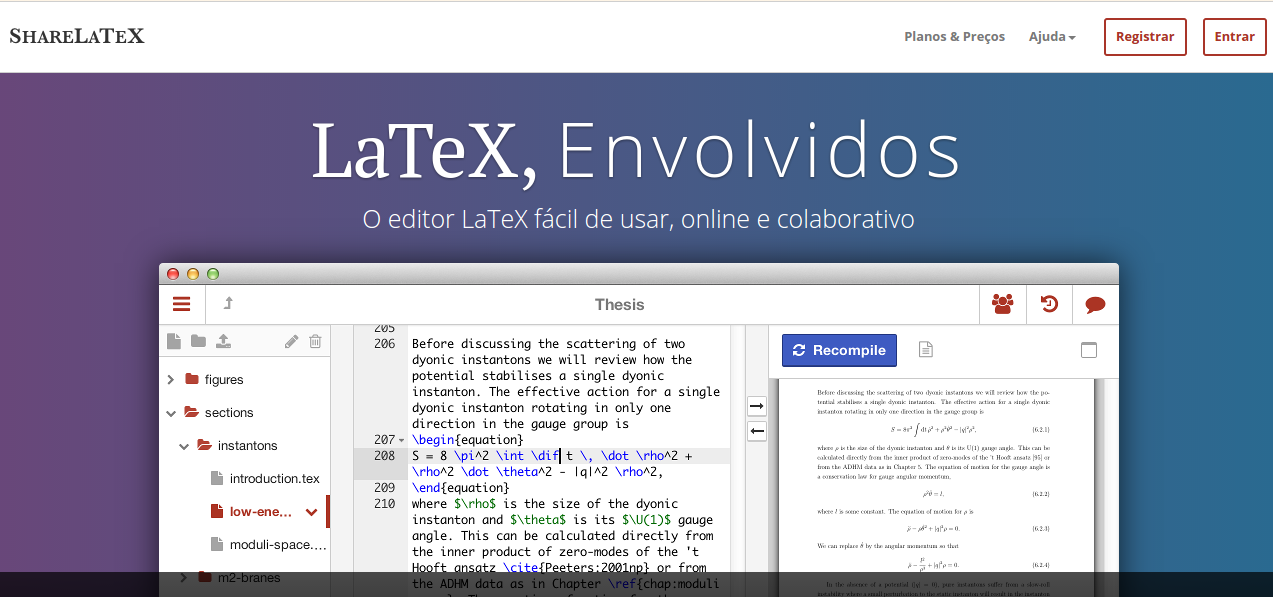
\includegraphics[scale=0.13]{Imagens/shareLatex}
  \caption{ShareLaTeX: \url{https://pt.sharelatex.com/}}
 \end{figure}
 \begin{figure}
  
\includegraphics[scale=0.13]{Imagens/writeLatex}
  \caption{WriteLaTeX: \url{https://www.writelatex.com/}}
 \end{figure}
\end{frame}

\begin{frame}{Material de consulta}
 
 \begin{figure}
  
\includegraphics[scale=0.20]{Imagens/ctan}
  \caption{\small CTAN - The Comprehensive \TeX~Archive Network: \url{http://www.ctan.org/}}
 \end{figure}

 \begin{itemize}
  \item Prof. Sadao Massago (UFSCAR): \url{http://www.dm.ufscar.br/profs/sadao/latex/}
 \end{itemize}
\end{frame}

\begin{frame}

% \begin{figure}
%  
\includegraphics[scale=0.4]{Imagens/lion}
%  \\
%  {\tiny CTAN lion drawing by Duane Bibby.}
% \end{figure}
 
\begin{center}
  
\includegraphics[scale=0.4]{Imagens/lion}
  \vspace{1ex}
  
  \Huge Muito obrigado!
 \end{center}
\end{frame}


 \section*{Referências Bibliográficas}
 \begin{frame}[allowframebreaks=0.8]{Referências Bibliográficas}
 \beamertemplatebookbibitems
 \begin{thebibliography}{Referências}
 \bibitem{reboucas:10} {Diogo Leite Rebouças, Luiz Paulo de Souza Medeiros}, {\it Mini-curso de \LaTeX}, 9º Seminário de Informática e Engenharia da Computação, Julho de 2010.
 \end{thebibliography}
 \end{frame}

\end{document}
